% Copyright 2002-2024 The University of Maryland Baltimore County (UMBC)
% 1000 Hilltop Circle, Baltimore, Maryland, 21250, USA
% https://www.csee.umbc.edu/

\documentclass[letter,10pt]{article}
\usepackage[breaklinks,pdfa=true,bookmarks=true,pdfdisplaydoctitle=true]{hyperref}
\hypersetup{
    unicode=false,          % non-Latin characters in Acrobat’s bookmarks
    pdftoolbar=true,        % show Acrobat’s toolbar?
    pdfmenubar=true,        % show Acrobat’s menu?
    pdffitwindow=false,     % window fit to page when opened
    pdfstartview={XYZ null null 1.00},    % disable zoom
    pdftitle={Problem Solving and Computer Programming Syllabus},    % title
    pdfauthor={Joshua Massey},     % author
    pdfsubject={UMBC CMSC104 Problem Solving and Computer Programming},   % subject of the document
    pdfkeywords={Computer Science, Programming, Problem Solving, CSEE}, % list of keywords
    pdfnewwindow=true,      % links in new PDF window
    colorlinks=true,       % false: boxed links; true: colored links
    linkcolor=red,          % color of internal links (change box color with linkbordercolor)
    citecolor=green,        % color of links to bibliography
    filecolor=magenta,      % color of file links
    urlcolor=cyan           % color of external links
}
\usepackage{graphicx}
\usepackage{fancyhdr}
\pagestyle{fancy}
\usepackage[letterpaper, margin=1in]{geometry}
\geometry{letterpaper}
\usepackage{parskip} % Disable initial indent
\usepackage{color,soul} % Highligher
\usepackage[normalem]{ulem} % Strikethrough with \sout{}

\definecolor{cadmiumgreen}{rgb}{0.0, 0.42, 0.24}

\renewcommand{\today}{\number \day \ \ifcase \month \or January\or February\or March\or %
April\or May \or June\or July\or August\or September\or October\or November\or %
December\fi \ \number \year} 

\usepackage[utf8]{inputenc}
\fancyhf{}
\renewcommand{\headrulewidth}{0pt} % Remove default underline from header package
% \rhead{CMSC 104 Section 01: Problem Solving and Computer Programming}
% \lhead{\begin{picture}(0,0) \put(-65,-8){
\includegraphics[width=1.1cm]{Images/UMBC-vertical}} \end{picture}}
% \cfoot{\thepage}
% \rfoot{Fall 2024
}
% \lfoot{CMSC 104 (Section 01)}
\fancyhead[L]{
    \makebox[\textwidth][s]{
        \begin{picture}(0,15){
\includegraphics[height=0.375in]{Images/UMBC-primary-logo-RGB.png}}
        \end{picture}
        \hspace{9.25cm} % Adjust space between image and text as needed
        \shortstack[r]{CMSC 104 (Section 01): \\Problem Solving and Computer Programming}
    }
}
\fancyfoot[C]{
    \makebox[\textwidth][s]{
        \thepage
        \hspace{5cm}
        Fall 2024

        \hspace{5cm}
        CMSC 104 (Section 01)
    }
}
%\AtEndDocument{\vfill \LaTeX \hfill}
\AtEndDocument{\hfill \vfill Last modified: \today}

\begin{document}

\textbf{Semester:} Fall 2024
\\
\textbf{Location:} Engineering 122A \\
\textbf{Time:} Tuesdays \& Thursdays 5:30 PM -- 6:45 PM \\\\
\textbf{Instructor:} Joshua E. Massey \\
\textbf{Email:} \href{mailto:joshua.massey@umbc.edu?Subject=[CMSC 104]}{joshua.massey@umbc.edu} \\
\textbf{Teaching Fellow:} TBD \\
% \textbf{Email:} \href{mailto:marcusd2@umbc.edu?Subject=CMSC104}{marcusd2@umbc.edu}

\subsection*{Office Hours}
\begin{itemize}
\item Approximately 30 minutes prior to class, if planned ahead.
\item At least 30 minutes after class, possibly longer on Tuesdays.
\item Virtual meeting by appointment. Schedule via email.
\item In Email: Anytime, and I will respond within 48 hours.
\end{itemize}

\section*{Course Description}
\paragraph{}This course is designed to provide an introduction to problem solving and computer programming that does not require prior programming experience. Elementary problem solving skills and algorithm development will be introduced. Students will be taught the basic use of a programming environment and basic programming constructs (including loops, control statements, functions, and arrays).

\paragraph{Note:}This course does not fulfill any of the computer science major requirements. Students who have taken and received transfer credit for, or who are taking concurrently any computer programming course in a high-level programming language, will not receive credit for CMSC 104. The list of such computer programming courses includes, but is not limited to AP Computer Science, CMSC 201, CMSC 202, and sections of CMSC 291 that cover programming topics.

The following is a list of the topics that will be covered:
\begin{itemize}
\item Introduction to Computer Organization and Architecture
\item Data Representation and Memory Usage
\item Algorithm Design
\item Programming in Python
\end{itemize}

\section*{Overall Course Objectives}
\paragraph{}After completion of this course, students will be able to:
\begin{itemize}
    \item explain the implications of basic concepts of computer organization and architecture on program design and implementation;
    \item design basic and intermediate programs to solve problems using fundamental programming constructs (variables, loops, branching, functions);
    \item implement Python programs from designs using a development environment (Google Colab -- \url{https://colab.research.google.com/});
    \item describe how data is represented in memory and the relationship of these representations to Python variable types;
    \item explain the concept of an object and use objects \& functions from libraries, including the graphics, file access, and string formatting libraries;
    \item describe the concept of an algorithm and be able to design simple algorithms, including recursive algorithms;
    \item explain applications of computation in their chosen field.
\end{itemize}

\section*{Course Textbook}
\paragraph{}The Python programming book is the textbook for this course, and there is assigned reading in the course \hyperlink{sec:sechedule}{schedule} below corresponding to chapters in this book.


\includegraphics[scale=0.7]{Images/PythonThirdFrontCover}

\paragraph{}\textbf{Python Programming: An Introduction} by John Zelle, Third Edition. Franklin, ISBN 978-1-59028-275-5. e-book available at \url{https://redshelf.com}.

\subsection*{Optional Book}
\paragraph{}\textit{Code to Joy} is a great book about programming in general, and discusses the topic in a non-textbook format. 

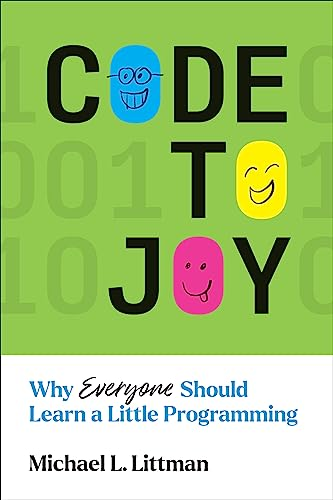
\includegraphics{Images/CodeToJoy}

\paragraph{}\textbf{Code to Joy: Why Everyone Should Learn a Little Programming} by Michael Littman. MIT, ISBN: 978-0-262-54639-3.

\section*{Course Work}\label{sec:coursework}
\paragraph{Attendance}It is important to be present for each class, though it's up to each individual student to best manage their own time. This is your time to have regular interaction with the instructor and Teaching Fellow, to ask questions, ask for specific examples, seek clarification, etc. I cannot overstate the importance of being able to ask questions and engage in dialog to help facilitate the learning process. \textbf{The students who end up being the most successful are the ones who regularly attend \underline{and} ask questions!}

\paragraph{Software}If you're using a Windows computer, you'll need to download and install Python from \href{https://www.python.org/downloads/windows/}{python.org}. If you have a Mac, Python is already installed, but you may want to install a newer version from \href{https://www.python.org/downloads/macos/}{python.org}. In both cases, make sure to install ``IDLE''. Additionally, you may wish to install PyCharm Community Edition from \url{https://www.jetbrains.com/pycharm/}. Both are free.

\paragraph{}A third option is to use Google Colabatory, available at \url{https://colab.research.google.com/} which doesn't require software installation.

\label{sec:cwhw}
\paragraph{Classwork \& Projects}Classwork will be submitted using Blackboard, and are due precisely one week after being assigned. For example, Classwork 1 is assigned on Wednesday, September 4\textsuperscript{th}, therefore the due date is 11:59 PM on Tuesday, September 19\textsuperscript{th}. Assignments may be completed early, but \underline{\hypertarget{sec:cwhw}{late assignments} will \textbf{not}} \underline{be accepted}\footnote{Late assignments may be accepted \textit{only} in the event of a documented extenuating circumstance.}. Projects are due two weeks after assignment. Classwork and Projects indicate the assignment \& due dates.

\paragraph{Quizzes}There are four quizzes and they will be held during the first 40 minutes of the class in which they're administered. The best ways to study for the quiz is to attend class, ask questions, and complete the assignments. Each quiz will focus on the materials since the quiz prior, including assigned readings, and will be \textit{cumulative}. Quizzes will be administered using the Respondus Lockdown Browser in Blackboard, so please read the following section for details on how to set it up and use it. There will be a practice quiz early in the semester to ensure everyone can use the system to ensure no surprises on quiz days.

\paragraph{LockDown Browser}This course uses the LockDown Browser for the quizzes and final exam. Watch this short video to get a basic understanding of LockDown Browser \url{http://www.respondus.com/products/lockdown-browser/student-movie.shtml}. Then download and install LockDown Browser from this link: \url{http://www.respondus.com/lockdown/download.php?id=978442813}. NOTE: This link is unique for UMBC. It cannot be used by non-UMBC students or websites outside of our campus. To take an online test, start LockDown Browser and navigate to the exam. You won't be able to access the exam with a standard web browser. For additional details on using LockDown Browser, review this FAQ \url{https://wiki.umbc.edu/x/BQb9Aw} or the Respondus Student Quick Start Guide (PDF) \url{http://respondus.com/products/lockdown-browser/guides.shtml#student}. Finally, when taking an online exam, follow these guidelines:
\begin{itemize}
\item Before starting the test, know how much time is available for it, and that you've allotted sufficient time to complete it;
\item Turn off all mobile devices, phones, etc. and place them in your bag, in the space designated by your instructor;
\item Remain at your desk or workstation for the duration of the quiz or exam;
\item LockDown Browser will prevent you from accessing other websites or applications; you will be unable to exit the test until all questions are completed and submitted.
\end{itemize}

\paragraph{Exams}There will be one exam, the final, which will also use the LockDown Browser. It is designed to reinforce the topics discussed throughout the semester in order to promote retention of the information.

\section*{Course Policies}
\subsection*{Grading}

\begin{center}
\begin{tabular}{ c c || c c}
\multicolumn{2}{c||}{\underline{Scale}} & \underline{Course Work} & \underline{Grade Distribution} \\
90\% - 100\% & A & Classwork & 15\% \\
80\% - 89\%  & B & Projects & 25\% \\
70\% - 79\%  & C & Quizzes & 30\% \\ 
60\% - 69\%  & D & Final Exam & 30\% \\
$<$60\%      & F & 
\end{tabular}
\end{center}

\paragraph{}For borderline grades, there may be adjustments in the student's favor based on attendance, but under no circumstances will the letter grades be lower than in the standard formula. Grades will not be ``curved'' in the sense that the percentages of A's, B's and C's are not fixed. As a guideline, a student receiving an ``A'' should be able to produce correct programs for the all of the assignments and quizzes with ease. As stated in the \hyperlink{sec:cwhw}{Classwork \& Projects} section, late work will not be accepted.

\subsection*{Academic Integrity}
\paragraph{}By enrolling is this course, each student assumes the responsibilities of an active participant in UMBC's scholarly community in which everyone's academic work and behavior are held to the highest standards of honesty. Cheating, fabrication, plagiarism, and helping others to commit these acts are all forms of academic dishonesty, and they are wrong. Academic misconduct could result in disciplinary action that may include, but is not limited to, suspension or dismissal. To find useful information about avoiding plagiarism infractions through appropriate citations, or to read the full policy regarding student academic misconduct for the graduate school, please see \url{http://www.umbc.edu/provost/integrity}.

\paragraph{}You are allowed \& \textit{encouraged} to discuss course materials with your peers! However, \underline{all assignments} \underline{are an individual effort!} Assignments will be checked for evidence of shared or copied code. If you have questions, or find that you are struggling, please ask questions, \underline{do not share code}\textbf{!}

\paragraph{}Please refrain from trying to find code online to help with your assignment. As stated a few times, if you are having trouble, then please ask for help during class, after class, or in an email. If you find yourself too tempted and do this anyway, include that URL in the assignment itself:
\begin{itemize}
\item Cite your source, don't claim it as your own,
\item If you can another student happen to use the same site and don't cite, that will be interpreted as cheating and a zero will be given for the assignment
\end{itemize}

\paragraph{Use of Generative Artificial Intelligence}You are strongly advised against using generative AI tools (like ChatGPT) in the course and generative AI use is prohibited in all assignments. This doesn't help you learn, and these tools (including ChatGPT) have been known to give incorrect responses. You learn by doing, making mistakes, figuring out how to fix the mistakes, and repeating. Being given potential incorrect answers is not learning. If you need help with the course material, please ask questions!

\newpage

\section*{* Tentative Schedule *}\label{sec:schedule}
\textit{Note: The schedule is subject to change. However, any changes will be thoroughly discussed and well disseminated. Please read the chapter \underline{before} class starts.}

% Fall schedule
\small
\begin{tabular}{c c l l l c}
Date    & Week & ~~~~~~~~~~~~Topic & Textbook & Code to Joy & Assignment \\ \hline
Th Aug 29  & 1  & Introduction, Syllabus Review & & & \sout{Quiz 0} \\ \hline
Tu Sept 3  & 2  & Computers and Programs & 1 & & \\
Th Sept 5  & 2  & Computers and Programs & & 1 & Classwork 1 \\
Tu Sept 10  & 3  & Writing Simple Programs & 2 & & \\
Th Sept 12 & 3  & Writing Simple Programs & & 2, 5 & Classwork 2 \\
Tu Sept 17 & 4  & Computing with Numbers & 3 & & Project 1\\
Th Sept 19 & 4  & Computing with Numbers & & & Classwork 3 \\
Tu Sept 24 & 5  & Objects and Graphics & 4 & & \\
Th Sept 26 & 5  & \hl{Quiz 1} & & & \\ \hline
Tu Oct 1 & 6  & Sequences & 5 & & \\
Th Oct 3   & 6  & Sequences & & 3 & Classwork 4 \\
Tu Oct 8   & 7  & Defining Functions & 6 & & Project 2\\
Th Oct 10   & 7  & Defining Functions & & 7 & Classwork 5 \\
Tu Oct 15  & 8  & Decision Structures & 7 & & \\
Th Oct 17  & 8  & \hl{Quiz 2} & & 4 & \\
Tu Oct 22  & 9  & Loops \& Booleans & 8 & & \\
Th Oct 24  & 9  & Loops \& Booleans & & 6 & Classwork 6 \\
Tu Oct 29  & 10 & Simulation \& Design & 9 & & \\
Th Oct 31  & 10 & Simulation \& Design & & & Classwork 7 \\ \hline
Tu Nov 5   & 11 & Defining Classes & 10 & & Project 3\\
Th Nov 7   & 11 & \hl{Quiz 3} & & & \\
Tu Nov 12  & 12 & Defining Classes & & & \\
Th Nov 14  & 12 & Data Collections & 11 & &  \\
Tu Nov 19  & 13 & Data Collections & & 8 & Classwork 8\\
Th Nov 21  & 13 & Object Oriented Design & 12 & & \\
Tu Nov 26  & 14 & Object Oriented Design & & & Classwork 9 \\
% Th Nov 27  & 14 & \hl{Quiz 4} & & & \\ \hline
           &    & \hl{Quiz 4} & & & \\ \hline
Tu Dec 3   & 15 & Algorithm Design \& Recursion & 13 & & \\
Tu Dec 5   & 15 & Algorithm Design \& Recursion & & 9 & Classwork 10 \\
Tu Dec 10   & 16 & Review & & & \\
Tu Dec 17  & 17 & \hl{Final Exam, 6:00 PM - 8:00 PM (Tentative)} & & & \\
\end{tabular}

% Spring schedule goes here

\section*{Accessibility \& Disability Accommodations, Guidance \& Resources}
\paragraph{}Accommodations for students with disabilities are provided for all students with a qualified disability under the Americans with Disabilities Act (ADA \& ADAAA) and Section 504 of the Rehabilitation Act who request and are eligible for accommodations. The Office of Student Disability Services (SDS) is the UMBC department designated to coordinate accommodations that creates equal access for students when barriers to participation exist in University courses, programs, or activities.

\paragraph{}If you have a documented disability and need to request academic accommodations in your courses, please refer to the SDS website at \url{sds.umbc.edu} for registration information and office procedures.
\begin{itemize}
\item SDS email: \href{mailto:disAbility@umbc.edu}{disAbility@umbc.edu}
\item SDS phone: \href{tel:+14104552459}{(410) 455-2459}
\end{itemize}
If you will be using SDS approved accommodations in this class, please contact the instructor to discuss implementation of the accommodations. During remote instruction requirements due to COVID, communication and flexibility will be essential for success.

\section*{Sexual Assault, Sexual Harassment, \& Gender Based Violence \& Discrimination}
\paragraph{}UMBC Policy\footnote{\url{https://ecr.umbc.edu/gender-discrimination-sexual-misconduct/}} in addition to federal and state law (to include Title IX) prohibits discrimination and harassment on the basis of sex, sexual orientation, and gender identity in University programs and activities. Any student who is impacted by sexual harassment, sexual assault, domestic violence, dating violence, stalking, sexual exploitation, gender discrimination, pregnancy discrimination, gender-based harassment, or related retaliation should contact the University’s Title IX Coordinator to make a report and/or access support and resources. The Title IX Coordinator can be reached at \href{mailto:titleixcoordinator@umbc.edu}{titleixcoordinator@umbc.edu} or \href{tel:+14104551717}{410-455-1717}.

You can access support and resources even if you do not want to take any further action. You will not be forced to file a formal complaint or police report. Please be aware that the University may take action on its own if essential to protect the safety of the community.

If you are interested in making a report, please use the \href{https://umbc-advocate.symplicity.com/titleix_report/index.php/pid364290?}{Online Reporting/Referral Form}.  Please note that, if you report anonymously, the University’s ability to respond will be limited.

\subsection*{Notice that Faculty and Teaching Assistants are Responsible Employees with Mandatory Reporting Obligations}

All faculty members and teaching assistants are considered Responsible Employees, per UMBC’s Policy on Sexual Misconduct, Sexual Harassment, and Gender Discrimination\footnote{\url{https://ecr.umbc.edu/policy-on-sexual-misconduct-sexual-harassment-and-gender-discrimination/}}. Faculty and teaching assistants therefore required to report all known information regarding alleged conduct that may be a violation of the Policy to the Title IX Coordinator, even if a student discloses an experience that occurred before attending UMBC and/or an incident that only involves people not affiliated with UMBC.  Reports are required regardless of the amount of detail provided and even in instances where support has already been offered or received.

While faculty members want to encourage you to share information related to your life experiences through discussion and written work, students should understand that faculty are required to report past and present sexual harassment, sexual assault, domestic and dating violence, stalking, and gender discrimination that is shared with them to the Title IX Coordinator so that the University can inform students of their \href{https://ecr.umbc.edu/rights-and-resources/}{rights, resources, and support}.  While you are encouraged to do so, you are not obligated to respond to outreach conducted as a result of a report to the Title IX Coordinator.

If you need to speak with someone in confidence, who does not have an obligation to report to the Title IX Coordinator, UMBC has a number of \href{https://ecr.umbc.edu/policy-on-sexual-misconduct-sexual-harassment-and-gender-discrimination/#confidential-resources}{Confidential Resources} available to support you:
\begin{itemize}
    \item \href{https://health.umbc.edu/}{Retriever Integrated Health} (Main Campus): \href{tel:+14104552472}{410-455-2472}; Monday – Friday 8:30 a.m. – 5 p.m.; For After-Hours Support, Call \href{tel:988}{988}.
    \item \href{https://shadygrove.umd.edu/student-affairs/counseling-well-being}{Center for Counseling and Well-Being} (Shady Grove Campus): \href{tel:+13017386273}{301-738-6273}; Monday-Thursday 10:00a.m. – 7:00 p.m. and Friday 10:00 a.m. – 2:00 p.m. (virtual) \href{https://shadygrove.titaniumhwc.com/}{Online Appointment Request Form}.
    \item Pastoral Counseling via \href{https://i3b.umbc.edu/spaces/the-gathering-space-for-spiritual-well-being/}{The Gathering Space for Spiritual Well-Being}: \href{tel:+14104556795}{410-455-6795}; \href{mailto:i3b@umbc.edu}{i3b@umbc.edu}; Monday – Friday 8:00 a.m. – 10:00 p.m.
\end{itemize}

Other Resources:
\begin{itemize}
    \item \href{https://womenscenter.umbc.edu/}{Women`s Center} (open to students of all genders): \href{tel:+14104552714}{410-455-2714}; \href{mailto:womenscenter@umbc.edu}{womenscenter@umbc.edu}; Monday – Thursday 9:30 a.m. – 5:00 p.m. and Friday 10:00 a.m. – 4 p.m.
    \item \href{https://ecr.umbc.edu/shady-grove-title-ix-resources/}{Shady Grove Student Resources}
    \item \href{https://ecr.umbc.edu/maryland-resources/}{Maryland Resources}
    \item \href{https://ecr.umbc.edu/national-resources/}{National Resources}
\end{itemize}

\section*{Child Abuse and Neglect\footnote{\url{https://ecr.umbc.edu/child-protection/}}}
Please note that Maryland law and UMBC policy\footnote{\url{https://education.umbc.edu/child-abuse-reporting-policy//}} require that faculty report all disclosures or suspicions of child abuse or neglect to the Department of Social Services and/or the police even if the person who experienced the abuse or neglect is now over 18.

\section*{Pregnant and Parenting Students}
UMBC’s Policy on Sexual Misconduct, Sexual Harassment and Gender Discrimination\footnote{\url{https://ecr.umbc.edu/policy-on-sexual-misconduct-sexual-harassment-and-gender-discrimination/}} expressly prohibits all forms of discrimination and harassment on the basis of sex, including pregnancy. Resources for pregnant, parenting and breastfeeding students are available through the University’s \href{https://ecr.umbc.edu/students/}{Office of Equity and Civil Rights}.  Pregnant and parenting students are encouraged to contact the Title IX Coordinator to discuss plans and ensure ongoing access to their academic program with respect to a leave of absence – returning following leave, or any other accommodation that may be needed related to pregnancy, childbirth, adoption, breastfeeding, and/or the early months of parenting.

In addition, students who are pregnant and have an impairment related to their pregnancy that qualifies as disability under the ADA may be entitled to accommodations through the \href{https://sds.umbc.edu/accommodations/registering-with-sds/}{Office of Student Disability Services}.

\section*{Religious Observances \& Accommodations}
UMBC Policy\footnote{\url{https://provost.umbc.edu/wp-content/uploads/sites/46/2022/08/Religious-Observance-Academic-Policy-2022_2023.pdf}} provides that students should not be penalized because of observances of their religious beliefs, and that students shall be given an opportunity, whenever feasible, to make up within a reasonable time any academic assignment that is missed due to individual participation in religious observances. It is the responsibility of the student to inform the instructor of any intended absences or requested modifications for religious observances in advance, and as early as possible. For questions or guidance regarding religious observances and accommodations, please contact the Office of Equity and Civil Rights at \href{mailto:ecr@umbc.edu}{ecr@umbc.edu}.

\section*{Hate, Bias, Discrimination and Harassment}
UMBC values safety, cultural and ethnic diversity, social responsibility, lifelong learning, equity, and civic engagement.

Consistent with these principles, UMBC Policy\footnote{\url{https://ecr.umbc.edu/discrimination-and-bias/}} prohibits discrimination and harassment in its educational programs and activities or with respect to employment terms and conditions based on race, creed, color, religion, sex, gender, pregnancy, ancestry, age, gender identity or expression, national origin, veterans status, marital status, sexual orientation, physical or mental disability, or genetic information.

Students (and faculty and staff) who experience discrimination, harassment, hate, or bias based upon a protected status or who have such matters reported to them should use the \href{https://umbc-advocate.symplicity.com/titleix_report/index.php/pid954154?}{online reporting/referral form} to report discrimination, hate, or bias incidents. You may report incidents that happen to you anonymously. Please note that, if you report anonymously, the University’s ability to respond may be limited.

\section*{Resources to Help you Succeed}
\paragraph{}UMBC’s Academic Success Center (ASC; \url{https://academicsuccess.umbc.edu/}) provides a range of resources to support students as they progress toward degree completion. Check out the following resources:

\begin{itemize}
\item Appointment Tutoring: The Academic Success Center offers free small group tutoring by appointment. Appointments can be scheduled online. To make an appointment, please visit \url{http://academicsuccess.umbc.edu/appointment-tutoring}

\item Computing Success Center: The Academic Success Center offers free drop-in tutoring for computer science courses through our Computing Success Center.\footnote{Though CMSC 104 is not specifically listed, any computer science tutor should be able to help with this course's content.}. 
 To see the schedule for this course, please visit \url{http://academicsuccess.umbc.edu/computing-success-center}

\item Academic Advocates: Advocates work one-on-one with students who need support navigating academic and institutional challenges, no matter how complex the concerns (i.e., personal, academic, or financial).  For more information, please visit \url{https://academicsuccess.umbc.edu/academic-advocacy/}

\end{itemize}

If you have a question, please contact the ASC at \href{mailto:academicsuccess@umbc.edu}{academicsuccess@umbc.edu}.
\end{document}
